\subsubsection{Sense}

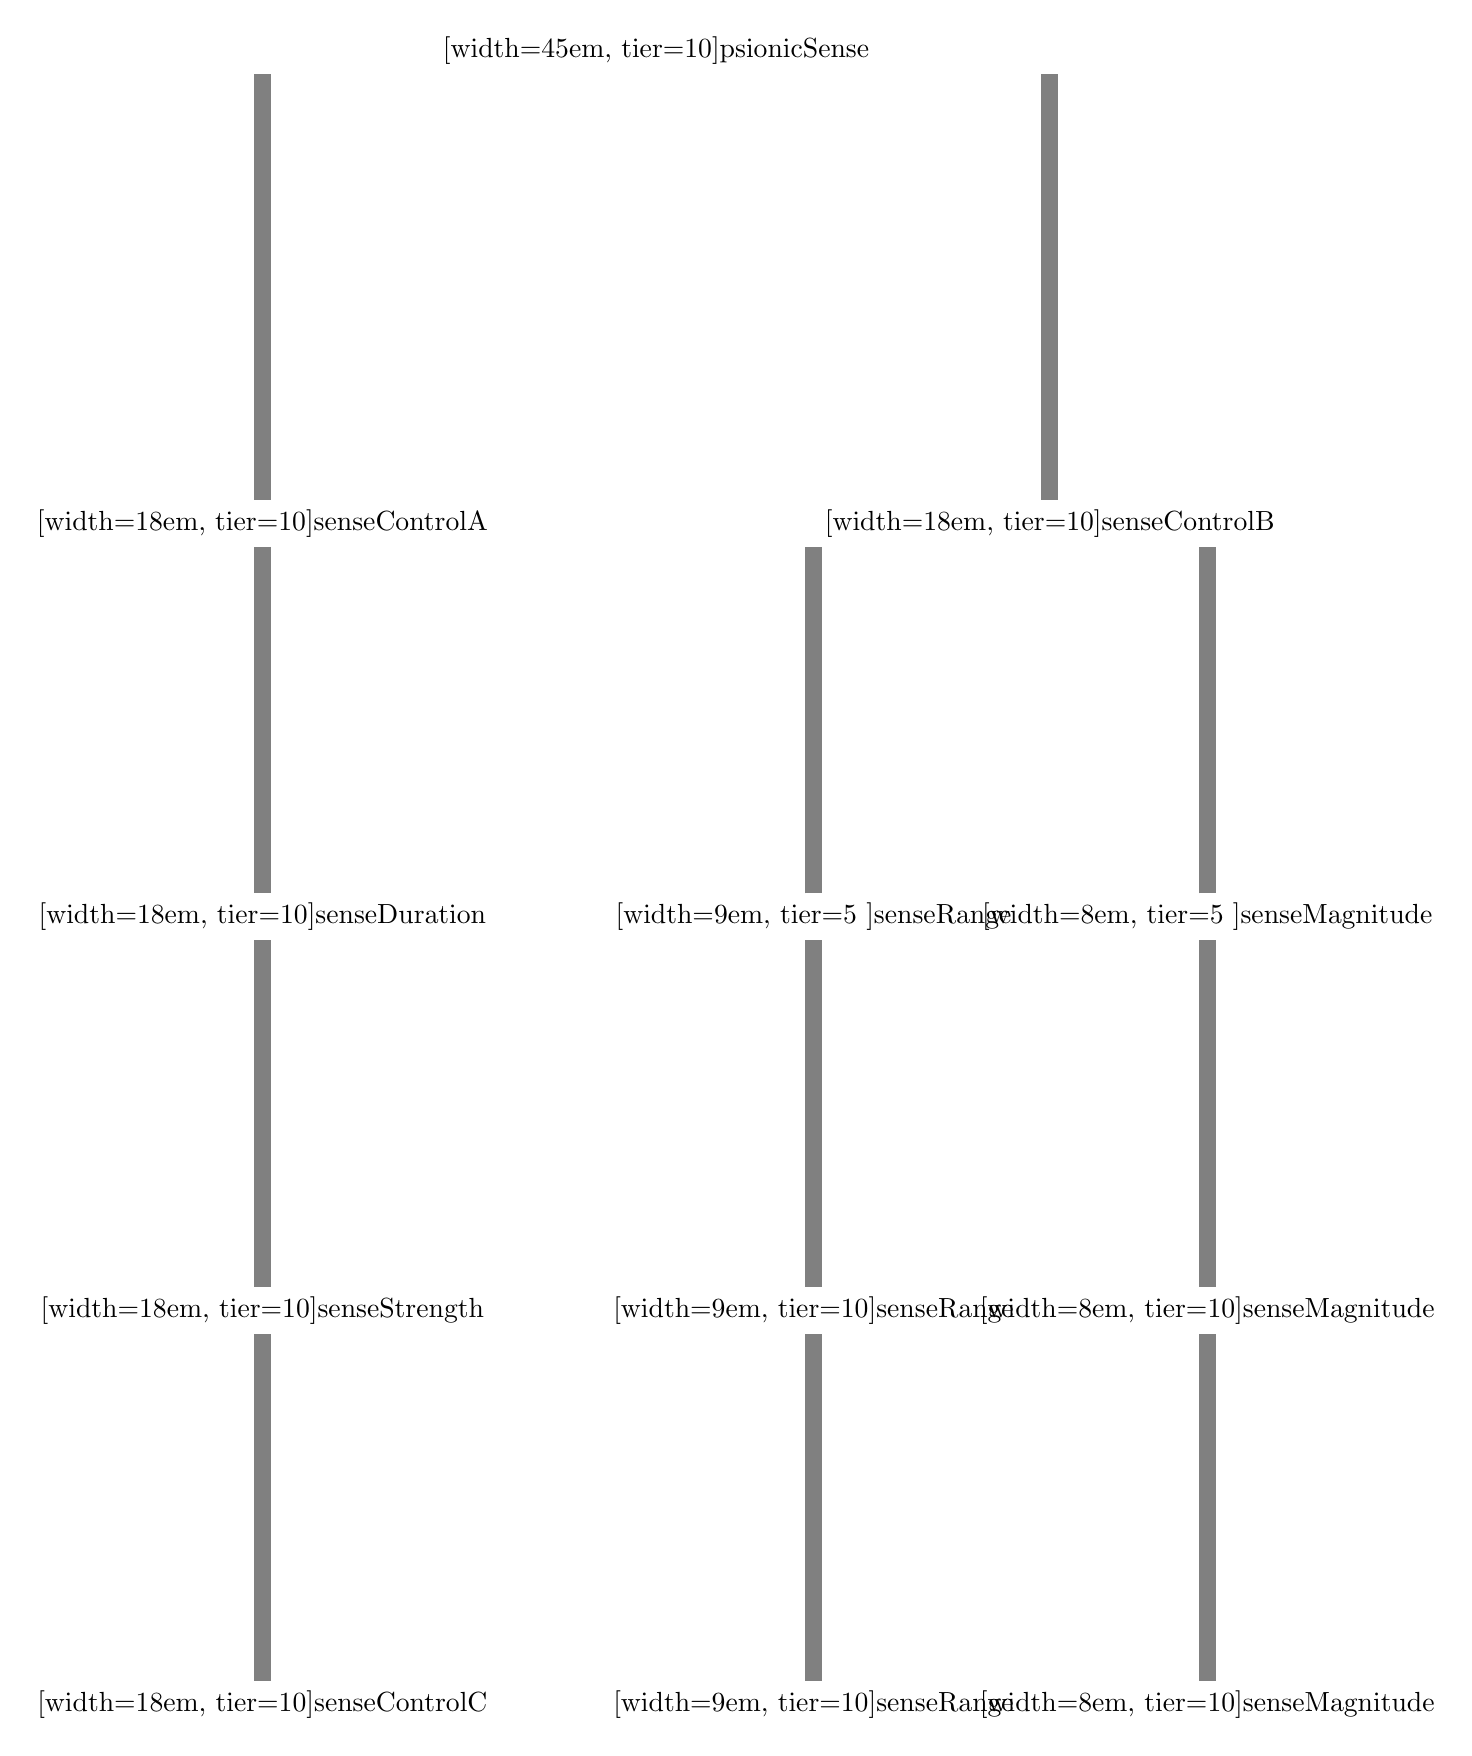
\begin{tikzpicture}
    \draw (-13,   6) node(pr){\TalentBox[width=45em, tier=10]{psionicSense}};
    \draw (-18,   0) node(ab){\TalentBox[width=18em, tier=10]{senseControlA}}
          (-8,    0) node(ad){\TalentBox[width=18em, tier=10]{senseControlB}}
          (-18,  -5) node(bb){\TalentBox[width=18em, tier=10]{senseDuration}}
          (-11,  -5) node(bc){\TalentBox[width=9em,  tier=5 ]{senseRange}}
          ( -6,  -5) node(bd){\TalentBox[width=8em,  tier=5 ]{senseMagnitude}}
          (-18, -10) node(cb){\TalentBox[width=18em, tier=10]{senseStrength}}
          (-11, -10) node(cc){\TalentBox[width=9em,  tier=10]{senseRange}}
          ( -6, -10) node(cd){\TalentBox[width=8em,  tier=10]{senseMagnitude}}
          (-18, -15) node(db){\TalentBox[width=18em, tier=10]{senseControlC}}
          (-11, -15) node(dc){\TalentBox[width=9em,  tier=10]{senseRange}}
          ( -6, -15) node(dd){\TalentBox[width=8em,  tier=10]{senseMagnitude}}
    ;

    \tikzstyle{bar}=[gray,-,>=stealth, line width=6pt]

    \draw [bar] (ab) -- (ab |- pr.south);
    \draw [bar] (ad) -- (ad |- pr.south);
    \draw [bar] (ab) edge (bb);
    \draw [bar] (bc) -- (bc |- ad.south);
    \draw [bar] (bd) -- (bd |- ad.south);
    \draw [bar] (bb) edge (cb);
    \draw [bar] (bc) edge (cc);
    \draw [bar] (bd) edge (cd);
    \draw [bar] (cb) edge (db);
    \draw [bar] (cc) edge (dc);
    \draw [bar] (cd) edge (dd);
\end{tikzpicture}
